\subsection{Decodificador BCD}

No sistema, apesar de ser possível representar diretamente cada dígito do display de 7 segmentos como uma combinação de sinais individuais (segmentos A a G), essa abordagem é ineficiente. Isso ocorre porque seriam necessários 7 bits para codificar apenas 10 estados válidos (0 a 9), resultando em desperdício de representação.

Para otimizar essa codificação, utiliza-se a representação em base binária. Com apenas 4 bits, é possível representar até 16 estados distintos ($2^4 = 16$), cobrindo com folga o intervalo necessário para os dígitos decimais.

No entanto, os valores binários não são diretamente compatíveis com o display de 7 segmentos. Portanto, é necessário um mapeamento entre a representação binária (BCD) e os segmentos físicos do display.

Esse mapeamento define quais segmentos devem ser ativados para cada número decimal.

Por exemplo, para o número 0, os segmentos ativos são A, B, C, D, E e F, enquanto o segmento G e dp permanecem desativados:

\begin{figure}[H]
    \centering
    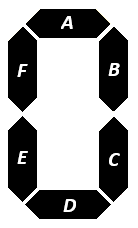
\includegraphics[width=0.15\linewidth]{images/zero-7seg.png}
    \caption{Representação do número 0 em um display de 7 segmentos.}
    \label{fig:zero-7seg}
\end{figure}

A tabela abaixo representa a codificação do número 0 no formato de segmentos:

\begin{center}
\begin{tabular}{c|cccccccc}
BCD & A & B & C & D & E & F & G & dp \\
\hline
0000 & 1 & 1 & 1 & 1 & 1 & 1 & 0 & 0 \\
\end{tabular}
\end{center}

Fazemos isso para os demais dígitos decimais, conforme apresentado na tabela completa abaixo:

\begin{center}
\begin{tabular}{c|cccccccc}
BCD & A & B & C & D & E & F & G & dp \\
\hline
0000  & 1 & 1 & 1 & 1 & 1 & 1 & 0 & 0 \\
0001  & 0 & 1 & 1 & 0 & 0 & 0 & 0 & 0 \\
0010  & 1 & 1 & 0 & 1 & 1 & 0 & 1 & 0 \\
0011  & 1 & 1 & 1 & 1 & 0 & 0 & 1 & 0 \\
0100  & 0 & 1 & 1 & 0 & 0 & 1 & 1 & 0 \\
0101  & 1 & 0 & 1 & 1 & 0 & 1 & 1 & 0 \\
0110  & 1 & 0 & 1 & 1 & 1 & 1 & 1 & 0 \\
0111  & 1 & 1 & 1 & 0 & 0 & 0 & 0 & 0 \\
1000  & 1 & 1 & 1 & 1 & 1 & 1 & 1 & 0 \\
1001  & 1 & 1 & 1 & 1 & 0 & 1 & 1 & 0 \\
1010  & - & - & - & - & - & - & - & -\\
1011  & - & - & - & - & - & - & - & -\\
1100  & - & - & - & - & - & - & - & -\\
1101  & - & - & - & - & - & - & - & -\\
1110  & - & - & - & - & - & - & - & -\\
1111  & - & - & - & - & - & - & - & -\\

\end{tabular}
\end{center}

\begin{figure}[H]
    \centering
    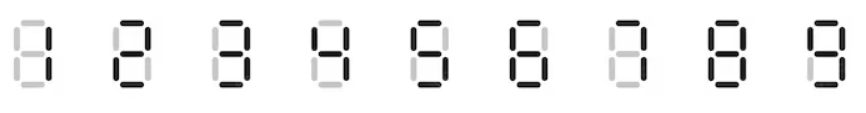
\includegraphics[width=0.8\linewidth]{images/numbers-7seg.png}
    \caption{Representação do números 1-9 em um display de 7 segmentos.}
    \label{fig:numbers-7seg}
\end{figure}

As combinações de 1010 a 1111 não representam dígitos válidos no sistema BCD, sendo tratadas como estados \textit{“don’t care”}, representados por "-" podendo assumir qualquer valor durante o processo de simplificação lógica.

A partir dessa tabela-verdade, é possível derivar oito funções booleanas independentes, uma para cada segmento (A até G) e uma adicional para o ponto decimal (dp).

Para isso, são utilizados 8 mapas de Karnaugh de 4 variáveis, permitindo a minimização das expressões booleanas associadas a cada uma das 8 saídas. Os quais, visto a extensão, foram disponibilizados separadamente, no github onde este trabahlo foi publicado (\url{https://github.com/Nick-Collin/Digital-Stopwatch-in-Minecraft}).

As funções resultantes descrevem o comportamento do decodificador BCD para display de 7 segmentos para todos os números de zero à nove.

\begin{align*}
A &= (\lnot N_{2} \land \lnot N_{0}) \lor N_{1} \lor (N_{2} \land N_{0}) \lor N_{3} \\[4pt]
B &= (\lnot N_{2}) \lor (\lnot N_{1} \land \lnot N_{0}) \lor (N_{1} \land N_{0}) \\[4pt]
C &= (\lnot N_{1}) \lor N_{0} \lor N_{2} \\[4pt]
D &= (\lnot N_{2} \land \lnot N_{0}) \lor (\lnot N_{2} \land N_{1}) \lor
(N_{2} \land \lnot N_{1} \land N_{0}) \lor (N_{1} \land \lnot N_{0}) \lor N_{3} \\[4pt]
E &= (\lnot N_{2} \land \lnot N_{0}) \lor (N_{1} \land \lnot N_{0}) \\[4pt]
F &= (\lnot N_{1} \land \lnot N_{0}) \lor (N_{2} \land \lnot N_{1}) \lor
(N_{2} \land \lnot N_{0}) \lor N_{3} \\[4pt]
G &= (\lnot N_{2} \land N_{1}) \lor (N_{2} \land \lnot N_{1}) \lor
N_{3} \lor (N_{1} \land \lnot N_{0}) \\[4pt]
dp &= 0
\end{align*}

Assim, montou-se o circuito do Decodificador BCD no Logisim: 

\begin{figure}[H]
    \centering
    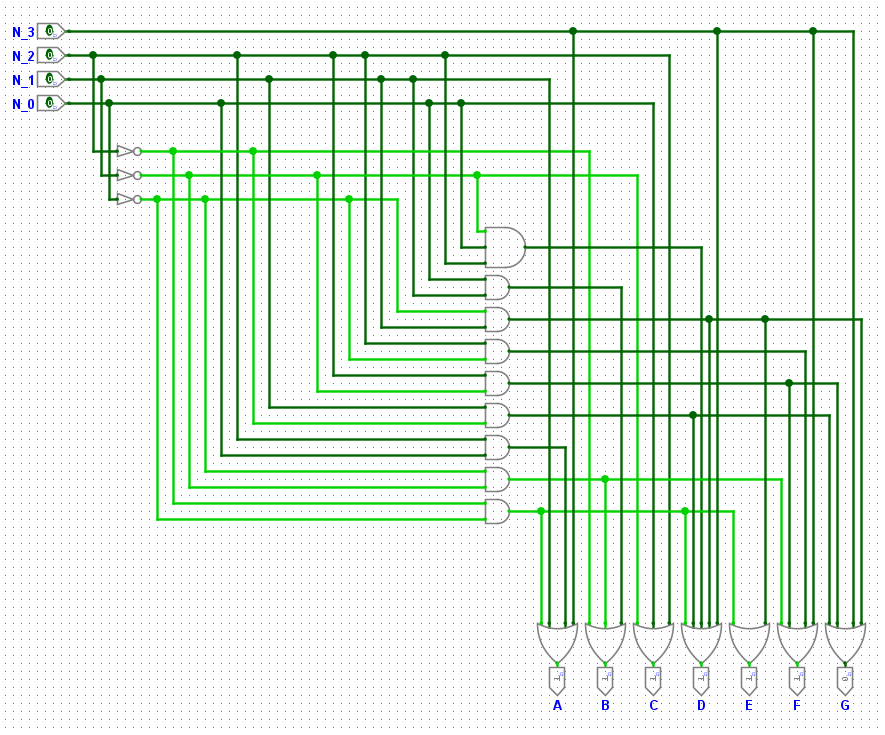
\includegraphics[width=0.7\linewidth]{images/BCD-decoder-circuit.png}
    \caption{Circúito digital do decodificador BCD no Logisim Evolution}
    \label{fig:BCD-decoder-circuit}
\end{figure}

Da mesma forma, traduziu-se o circúito para o Minecraft, diretamente ligado a uma unidade de display 7 segmentos: 

\begin{figure}[H]
    \centering
    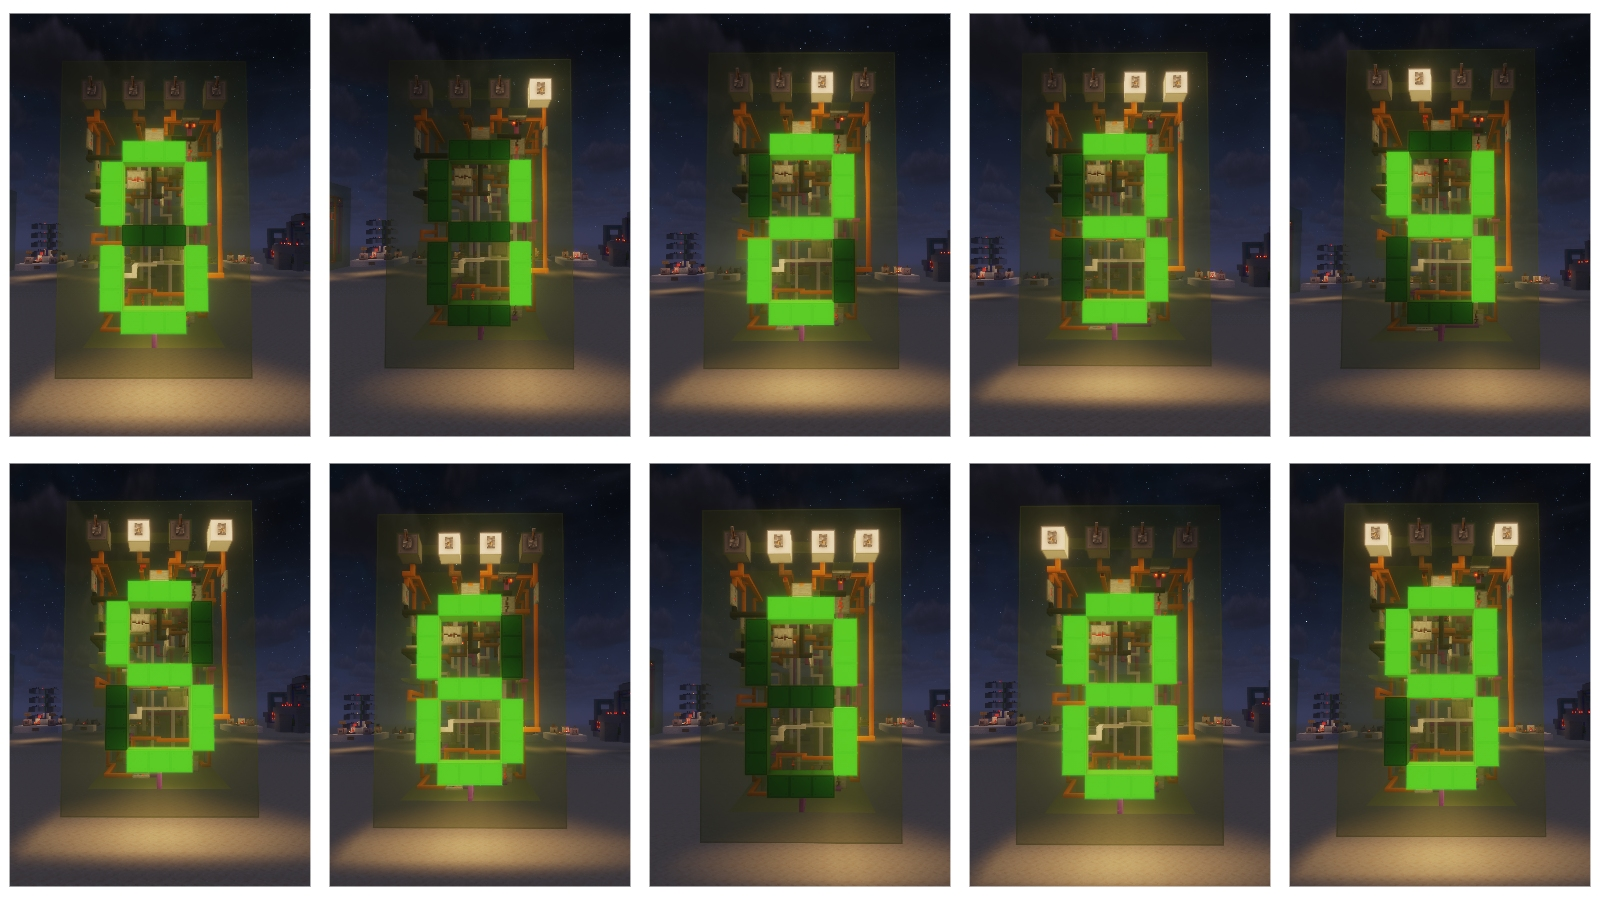
\includegraphics[width=0.7\linewidth]{images/nums-0-9-redstone7seg.jpg}
    \caption{Números 0-9 no Decodificador BCD em redstone}
    \label{fig:nums-0-9-redstone7seg}
\end{figure}

Este workflow, no qual idealizamos uma função, produzimos a tabela verdade, resolvemos os $n$ mapas de Karnough para cada uma das $n$ saídas, implementamos o circpuito no Logisim e depois no Minecraft tornará a aparecer diverssas vezes ao longo deste documento.